\chapter{Reducing special ILPs to Shortest Path}
\section{Problem statement}
In their book \textit{Algebraic statistics for computational biology} \cite{algebraic_statistics}, the authors briefly mention an algorithm to solve integer linear programs by constructing a certain graph and solving the shortest path problem between two specifically chosen vertices. The resulting path will dictate the solution vector, and the length of that path will represent the value of that solution. Initially, this approach was restricted to matrices whose columns all sum up to the same number. In this chapter, we aim to revisit and rigorously explain this result. Furthermore, to enhance the practical feasibility of this algorithm, we will present some ideas to accelerate its execution.

\section{Solving Shortest Path using Dijkstra's Algorithm}
Before delving into the translation of Integer Linear Programs (ILPs) to a shortest path problem, let's revisit the fundamental concept of finding the shortest path in a graph. Dijkstra's algorithm stands as a cornerstone in graph theory, offering a systematic approach to determine the shortest path between nodes in a weighted graph \cite{introduction_to_algorithms}. It works by iteratively selecting the vertex with the shortest distance from the source and relaxing its outgoing edges. Here's how it works:

\subsection{Algorithm}
Given a weighted graph $G = (V, E)$ with vertices $V$ and edges $E$, and two specified vertices $s$ (source) and $t$ (target), we aim to find the shortest path from $s$ to $t$. Let $w(u, v)$ denote the weight of the edge from vertex $u$ to vertex $v$.

\begin{enumerate}
    \item Initialize a priority queue $Q$ and an array $dist$ to keep track of the shortest distance from the source vertex $s$ to every other vertex in the graph. Initially, set $dist[v] = \infty$ for all vertices $v$, except for $dist[s] = 0$.
    \item Enqueue the source vertex $s$ into the priority queue $Q$ with priority $0$.
    \item While $Q$ is not empty:
    \begin{enumerate}
        \item Dequeue a vertex $u$ with the minimum priority from $Q$.
        \item For each neighbor $v$ of $u$:
        \begin{enumerate}
            \item Calculate the potential new shortest distance to $v$ as $new\_dist = dist[u] + w(u, v)$.
            \item If $new\_dist < dist[v]$, update $dist[v]$ to $new\_dist$ and enqueue $v$ into $Q$ with priority $new\_dist$.
        \end{enumerate}
    \end{enumerate}
    \item Once the target vertex $t$ is dequeued from $Q$, the shortest path has been found, and the shortest distance to $t$ is $dist[t]$.
\end{enumerate}

\subsection{Pseudocode}
Here's the pseudocode for Dijkstra's algorithm:

\begin{verbatim}
function Dijkstra_Shortest_Path(G, s, t):
    dist = array of size |V| with all elements set to infinity
    dist[s] = 0
    Q = priority queue initialized with (s, 0)
    
    while Q is not empty:
        u, priority = Q.dequeue_min()
        if u == t:
            return dist[t]  // Shortest distance found
        for each neighbor v of u:
            new_dist = dist[u] + w(u, v)
            if new_dist < dist[v]:
                dist[v] = new_dist
                Q.enqueue(v, new_dist)
    return "No path found"
\end{verbatim}

\subsection{Runtime Analysis}
The runtime complexity of Dijkstra's algorithm is $O((|V| + |E|) \log |V|)$ using a binary heap priority queue implementation. This makes it efficient for finding the shortest path in large, weighted graphs.


\section{Reduction}
\subsection{Definitions and preparation}
As mentioned above, we will exclusively be handling matricies who's columns all sum up to the same number. As this is a mouth full to say (and write), let's define an abbrviation:

\begin{definition}
    \label{def:CCS}
    Let $\mathbb{K}$ be a field and $\alpha \in \mathbb{K}$. Let $S_{\alpha}(\mathbb{K}^{m \times n})$ be the set of matricies of size $m \times n$, who's column all sum up to $\alpha$, namely:
    $$S_{\alpha}(\mathbb{K}^{m \times n}) := \{A \in \mathbb{K}^{m \times n}\mid \forall j \in [n]\colon \sum_{i=1}^{m} A_{ij} = \alpha\}$$
    We will call these matricies \textbf{CCS matricies}, for \textbf{C}onstant \textbf{C}olumn \textbf{S}um.
\end{definition}

At the core of ILPs lies always a system of linear equation $A \vec x = \vec b$. It is crucial to understand that if $A$ is a CCS matrix, all solutions $\vec x$ have certain properties, as described in the first lemma. This will be the key to constructing the graph, our goal. 

\begin{lemma}
    \label{lemma:ilp_pre1}
    Let $A\in S_\alpha(\N^{m \times n})$, $\alpha > 0$. Let $\vec b \in \N^m$ arbitrary and consider the linear system of equation $A\vec x=\vec b$, where $\vec x \in \N^n$. Then, the following two statements are true

    \begin{enumerate}
        \item[(1)] For all solutions $\vec x \in \N^n$ must hold that its components must always sum up to the same number $k$.
        \item[(2)] There only exist a solution of the components of $b$ sum up to a multiple of $\alpha$. This multiple turnes out to be $k \cdot \alpha$.
    \end{enumerate}
\end{lemma}

\begin{proof}
    Let's assume there exists a solution $\vec x \in \N^n$ of the linear system of equation $A\vec x=\vec b$.
    $$\sum_{i=1}^m b_i = \sum_{i=1}^{m}\sum_{j=1}^{n}A_{ij} x_j = \sum_{j=1}^{n}\underbrace{\sum_{i=1}^{m}A_{ij}}_\alpha x_j = \alpha \cdot \sum_{j=1}^{n}x_j$$
    Because $\alpha$ and $b_i$ are fixed and will not change dependent of $\vec x$ and $\alpha \neq 0$, statement (1) immidiatly follows. Thus we have proven, if there exist a solution $\vec x \in \N^n$, then it must hold that $\sum_{i=1}^{m}b_i = \alpha \cdot k$, which is the contraposition of (2).
\end{proof}


\subsection{Construction the graph}
We want to be able to solve an ILP by using the shortest path framework. The main task is to build a weighted, directed graph $G = (V, E)$ based on an ILP. As mentioned before, we will only look at ILPs who's matrix is a CCS matrix. Let $(A \in S_\alpha(\N^{m \times n}), \vec b \in \N^m, \vec\omega \in \Z^n), \alpha > 0$ be our ILP. Let $k := \frac{1}{\alpha} \sum_{i=1}^{n}b_i \in \N$. Because of lemma \ref{lemma:ilp_pre1}, $k \in \N$. Now we can build the set of vertecies $V$. The resulting graph consists of $k$ layers of vertecies. We will call the layers $V_i, i \in [k]$. Thus $V := V_1 \cup \dots \cup V_k$. Each vertex will be represented by some vector:
$$V_i := \left\{A\vec x \mid \vec x \in \N^n, \sum_{j=1}^{n} x_j = i \right\}$$ 
It is clear that $V_0 = \{\vec 0\}$ and if $A\vec x = \vec b$ has solutions, we know from lemma \ref{lemma:ilp_pre1} that $\vec b \in V_k$. 

Edges, will only exist between consecutive layers. The basic idea is, that the underlying connected vectors $\vec x, \vec x'$ will differ by some unit vector $\hat e$ ($\vec x' = \vec x + \hat e$). Only if this is true, the vertecies $A\vec x$ and $A\vec x'$ are connected. This can of cause only happen for vertecies in consecutive layers. More formally: 
$$E := \{(u, v) \in V^2\mid \exists \hat e \in \{\hat e_1, \dots, \hat e_n\}\colon v = u + A\hat e\}$$

The last steps is defining the weights of the graph. Remember that every edge corresponds to adding some unit vector. The dot-product of this unit vector and the weights vector will be the weight of that edge:
$$w(v, v + A\hat e_i) := \sprod{\vec \omega}{\hat e_i}$$

Now consider a path beween $\vec 0\in V_0$ and $\vec b \in V_k$. As edges only exist between consecutive layers, the path will always traverse exactly $k$ edges and therby visit all $k+1$ layers once.

The next lemma will link paths in $G$ to our ILP, which will be essential when understanding why the shortest path solves our ILP.

\begin{lemma}
    Let $V, E, w, (A, \vec b, \vec \omega)$ be as in this chapter. Let $v \in V$ be a vertex of $G$. For any vector $\vec x \in \N^n$ such that $A\vec x = v$ there will be a path $P$ from $\vec 0$ to $v$ in $G$ such that the weight of $P$ is equal to $\sprod{\vec\omega}{\vec x}$. 
\end{lemma}
\begin{proof}
    We will prove, that this fact is true for any node in layer $i$, by induction over $i$. 
    
    The base case is $i=0$, hence we only have to consider $V_0$. We already know that $V_0 = \{\vec0\}$. So let $v := \vec 0$. The only vector $\vec x$ such that $A\vec x = v$ is $\vec x = \vec 0$, the column sums in $A$ are strictly positive. Thus $\sprod{\vec x}{\omega} = 0$ and the only path from $\vec 0$ to $\vec 0$ is the empty path with weight 0. Tadaa
    
    Let the statement be true for some $i < k$. We will proof it for $i+1$. Let $v \in V_{i+1}$ and $\vec x \in \N^n$ such that $A\vec x = v$. We know that $\sum_{j=1}^n x_j = i+1$. Let $\hat e$ be a basis vector such that $\vec x - \hat e =: \vec x' \in \N^n$. We know that $\sum_{j=1}^{n} x'_i = i+1-1=i$ and hence $A\vec x' \in V_i$. Thus by assumption there exists a path $P'$ from $\vec 0$ to $v' := A\vec x'$ such that its weight is $\sprod{\vec \omega}{\vec x'}$. Because $\vec x$ and $\vec x'$ only differ by a unit vector $\hat e$, the edge $(v', v)$ exists with weight $A\hat e$. So we can consider the path $P := P' \circ (v', v)$. It connects $\vec 0$ and $v$. And has the weight of $P'$ plus the weight of the edge, thus the weight $\sprod{\vec \omega}{\vec x'} + \sprod{\vec\omega}{\hat e} = \sprod{\vec \omega}{\vec x' + \hat e} = \sprod{\vec \omega}{\vec x}$. Which proves what we wanted to show.
\end{proof}

Looking at all paths from $\vec 0$ to $\vec b$ and then considering their weights is thus equivilant to looking at all solution to $A\vec x = \vec b$ and considering all values $\sprod{\vec\omega}{\vec x}$. The shortest path represents the smalles of those values. Hence solving shortest path between $\vec 0$ and $\vec b$ will yield a path who's weight is the optimal value for $\sprod{\vec\omega}{\vec x}$.\qed
\begin{figure}
    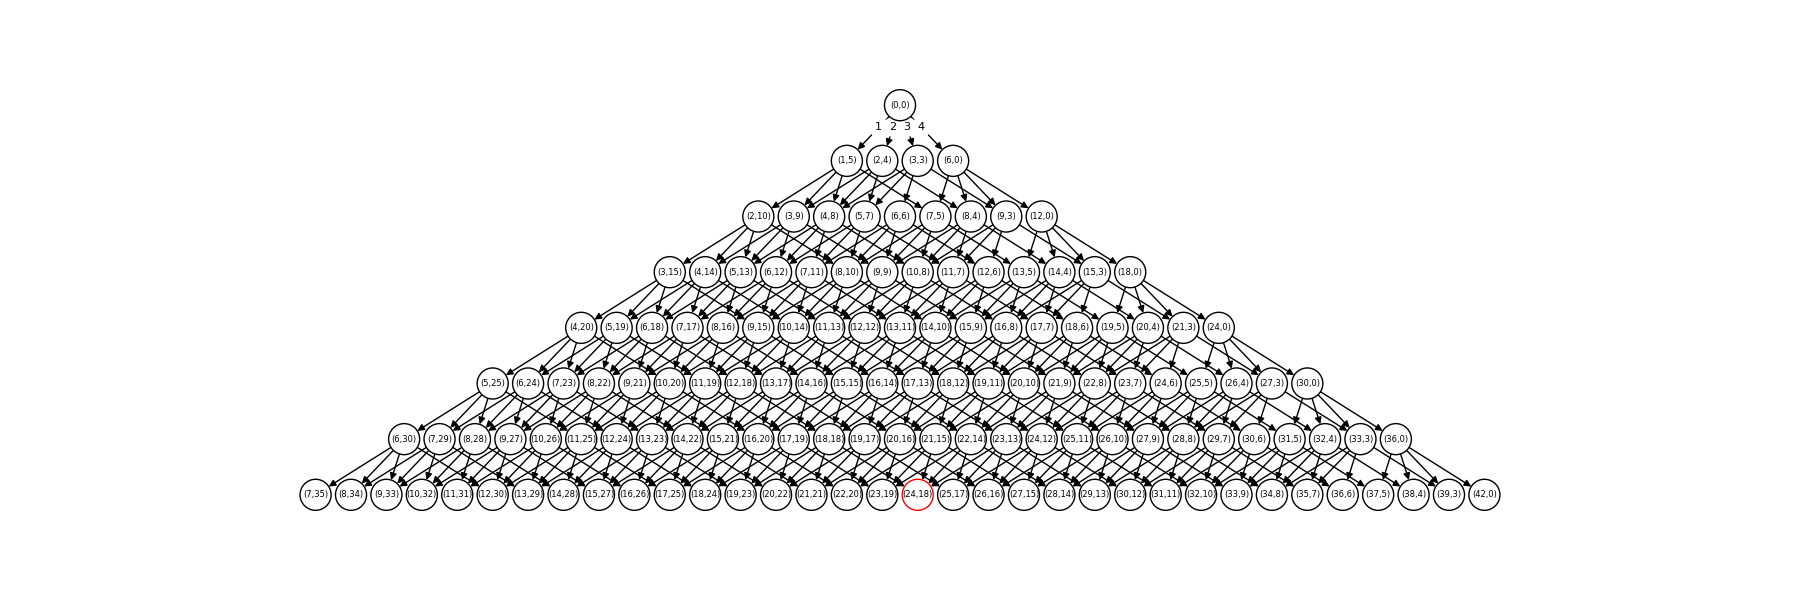
\includegraphics[width=\columnwidth]{ILP2graph.png}
    \caption{\label{fig:ILP2graph_no_optimisation}The graph for the ILP: $A = \smat{1&2&3&6\\5&4&3&0}, \vec b = \smat{24\\18}, \vec \omega = \smat{1\\2\\3\\4}$. All weights after the first layer are hidden.}
\end{figure}

An example of this graph construction can be viewed in figure \ref{fig:ILP2graph_no_optimisation}

\section{Immediate optimisation ideas}
As you can see, the graphs get big very quickly. Of cause this is the direct consequence of the NP-hard nature of ILPs. But we must not give up immediatly. There are a few things we can do to easily shrink down the size of that graph. First, observe that the entries in the vertex vectors can only grow. This means, if at least one entry is is bigger as the corresponding entry in $\vec b$, we can remove this node or just stop considering it in Dajkstra. When removing all those nodes, with bigger entries, we arrive at a much smaller graph, which can be seen in figure \ref{fig:ILP2graph_no_big_entries}.

\begin{figure}
    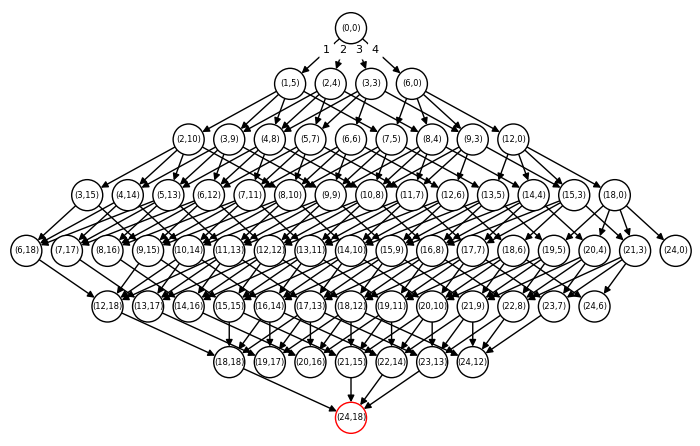
\includegraphics[width=\columnwidth]{ILP2graph_no_big_entries.png}
    \caption{\label{fig:ILP2graph_no_big_entries}The graph for the ILP: $A = \smat{1&2&3&6\\5&4&3&0}, \vec b = \smat{24\\18}, \vec \omega = \smat{1\\2\\3\\4}$. All weights after the first layer are hidden. All vertecies have been removed, where at least one component is bigger than the corresponding one in $\vec b$}
\end{figure}

Aside from removeing vertecies we can also remove some edges. To see that, let us consider the node $A(\hat e_1 + \hat e_2)$. We know, that it exists in layer 2. We can see that they are at least 2 paths to this node $\vec 0 \rightarrow A\hat e_1 \rightarrow A(\hat e_1 + \hat e_2)$ and $\vec 0 \rightarrow A\hat e_2 \rightarrow A(\hat e_1 + \hat e_2)$. And both paths will have the same weight, namely $\sprod{\vec \omega}{\hat e_1 + \hat e_2}$ and also respresent the same vector $\hat e_1 + \hat e_2$. That there exists 2 paths for one vector is redundant and influences negatively the performence of the shortest path execution. We can remove these duplicate paths by remembering which unit vector we added, let that be $\hat e_i$ previously and only add unit vectors $\hat e_j$ with $j \geq i$ to construct edges. Then the edge $(A\hat e_2, A(\hat e_1 + \hat e_2))$ would not exists and thus the duplicate path would be removed. If you do that to the original graph, you arrive at figure \ref{fig:ILP2graph_unique_paths}

\begin{figure}
    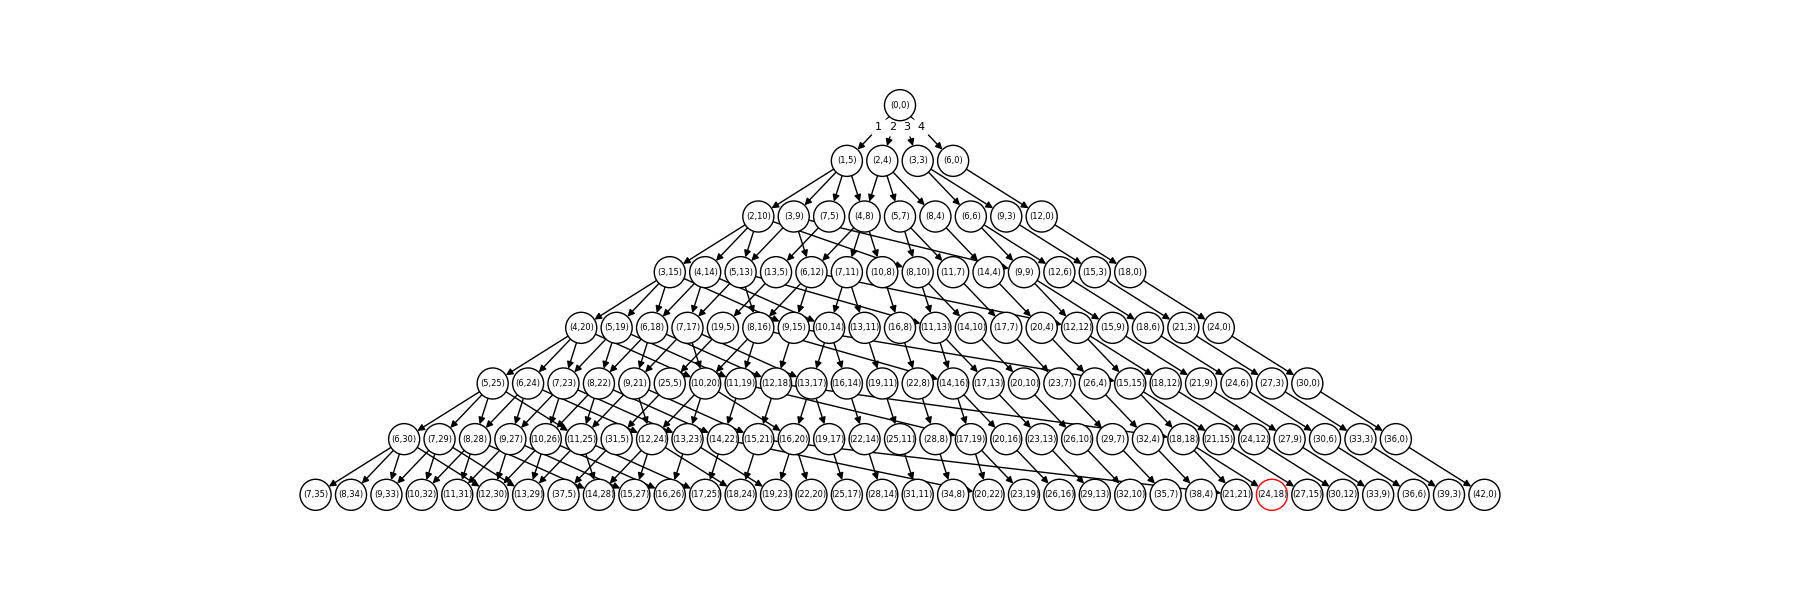
\includegraphics[width=\columnwidth]{ILP2graph_unique_paths.png}
    \caption{\label{fig:ILP2graph_unique_paths}The graph for the ILP: $A = \smat{1&2&3&6\\5&4&3&0}, \vec b = \smat{24\\18}, \vec \omega = \smat{1\\2\\3\\4}$. All vectors $\vec x$ now correspond with an \textit{unique} path from $\vec 0$ to $A\vec x$.}
\end{figure}

We have seen an option to remove vertecies and an option to remove edges. But we must not apply those 2 optimisations seperatly, but we can also combine them. The result drstically reduces the size of the graph, as seen in figure \ref{fig:ILP2graph_unique_paths_and_no_big_entries}

\begin{figure}
    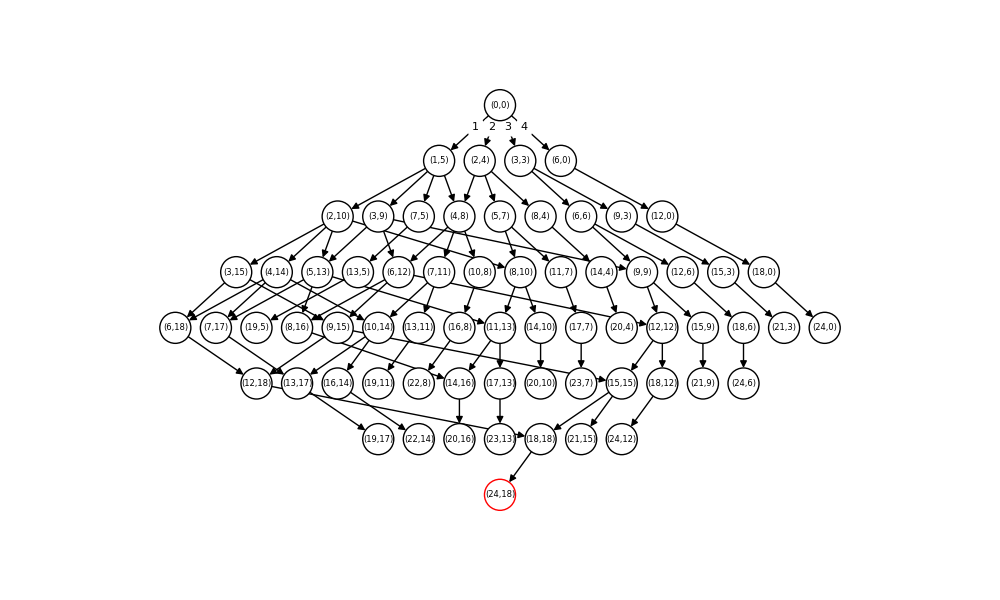
\includegraphics[width=\columnwidth]{ILP2graph_unique_paths_and_no_big_entries.png}
    \caption{\label{fig:ILP2graph_unique_paths_and_no_big_entries}The graph for the ILP: $A = \smat{1&2&3&6\\5&4&3&0}, \vec b = \smat{24\\18}, \vec \omega = \smat{1\\2\\3\\4}$. Unique paths and big components removed.}
\end{figure}

Looking at the final result in figure \ref{fig:ILP2graph_unique_paths_and_no_big_entries} one might say, that it would be benificial to now remove the vertecies with no children. And yes, that would further shrinken the graph. The problem with that optimisation is, that this couldn't be done on the fly within the Dajkstra algorithm. The vertecies can be discarded when visited and the edges can also be discarded while handling a vertex. But whether a vertex has children or not cannot be known a priori. Nevertheless, I included the graph, when we iteratively – bottom-up – remove all nodes without children to better understand the graph, see figure \ref{fig:ILP2graph_unique_paths_and_no_big_entries_and_no_leaves}.

\begin{figure}
    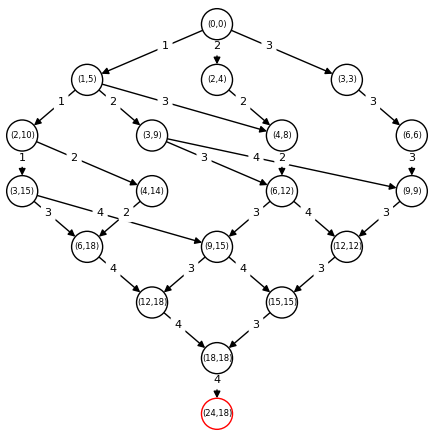
\includegraphics[width=\columnwidth]{ILP2graph_unique_paths_and_no_big_entries_and_no_leaves.png}
    \caption{\label{fig:ILP2graph_unique_paths_and_no_big_entries_and_no_leaves}The graph for the ILP: $A = \smat{1&2&3&6\\5&4&3&0}, \vec b = \smat{24\\18}, \vec \omega = \smat{1\\2\\3\\4}$. Unique paths and big components removed and all childrenless vertecies removed.}
\end{figure}

From this manageble representation, we can read of the solution of the ilp. The path with the lowest weight is the path on the outer left of graph. This path corresponds to $\vec x = \hat e_1 + \hat e_1 + \hat e_1 + \hat e_3 + \hat e_4 + \hat e_4 + \hat e_4 = (3, 0, 1, 3)^\top$ and indeed $A\vec x = \vec b$. 


% Nicht mehrere Pfade frü einen Vektor
% Wenn einträge zu groß werden discarden
% Kinderlose löschen
